\documentclass{article}
\usepackage{C:/Users/guitr/Documents/git_repositories/tpack/tpack}
% \usepackage{C:/Users/Admin-PC/Documents/git_repository/tpack/tpack}
% \usepackage{/home/tr0fin0/git_repositories/tpack/tpack}
% \usepackage{/home/Documents/git_repositories/tpack/tpack}
\usetikzlibrary{decorations.pathreplacing,calligraphy}

\title{OI201 - Systèmes d'Exploitation}
\project{Résumé Théorique}
\author{Guilherme Nunes Trofino}
\authorRA{2022-2024}


\makeatletter
\begin{document}\selectlanguage{french}
\maketitle
\setlength{\parindent}{0pt}

\newcommand{\comparison}[2]{
    \begin{remark}
        On considère les caractéristiques suivants:
        \begin{center}
            \begin{minipage}[t]{0.495\textwidth}
                \textbf{Avantages}:
                \begin{enumerate}[noitemsep]
                    #1
                \end{enumerate}
            \end{minipage}
            \begin{minipage}[t]{0.495\textwidth}
                \textbf{Inconvénients}:
                \begin{enumerate}[noitemsep]
                    #2
                \end{enumerate}
            \end{minipage}
        \end{center}
    \end{remark}
}


\newpage\tableofcontents

\section{Introduction}
\subfile{C:/Users/guitr/Documents/git_repositories/classes_ensta/intro.tex}
% \subfile{C:/Users/Admin-PC/Documents/git_repository/classes_ensta/intro.tex}
% \subfile{/home/tr0fin0/git_repositories/classes_ensta/intro.tex}
% \subfile{/home/Documents/git_repositories/classes_ensta/intro.tex}


\subsection{Information Matier}
\paragraph{Référence}Dans cette matière le but sera de comprendre comment une Système d'Exploitation marche.

\subsection{Histoire}
Les premières ordinateurs faisaient du \textbf{Batch Processing} à cause de la simplicité des systèmes de l'époque.
\begin{definition}\label{def:batchProcessing}
    Ordinateurs que n'exécutent qu'un seul programme à la fois font du \textbf{Batch Processing}. Dans ce cas le programme n'a pas besoin de partage les resources de l'ordinateur. Il pourrait acceder:
    \begin{enumerate}[noitemsep]
        \item toute la mémoire;
        \item tout le processeur;
        \item tous les périphériques;
    \end{enumerate}
\end{definition}
Comme ça n'est plus le cas actuellement on considère souvent le suivant:
\begin{phrase}
    un système d'exploitation n'est utile que lorsqu'il y a plusieurs programmes
\end{phrase}

\section{Architecture}

Souvent, pour comprendre comment l'ordinateur marche, c'est nécessaire de connaître sa structure physique nommé: 
\subsection{Architecture Matérielle}
\begin{definition}\label{def:architectureMaterielle}
    Décrit l'agencement interne de composants électroniques ainsi que leurs interactions.

    \begin{phrase}
        représente tous les ressources physiques disponibles et accessibles de l'ordinateur
    \end{phrase}
\end{definition}
Comment une ordinateur a plusieurs parties et le but de ce cours n'est pas de connaître tout on va considère une version très simplifiée d'un ordinateur.

\subsubsection{Architecture Von Neumann}
\begin{definition}\label{def:architectureVonNeumann}
    Architecture en que la mémoire est unique et utilisée pour stocker les instructions et les données des programmes.

    \begin{figure}[H]
        \centering\begin{tikzpicture}[]
            % modules
            \node[module] (CPU) {CPU};
            \node[module, right=of CPU] (MPU) {MPU};
            \node[module, right=of MPU] (BUS) {BUS};
            \node[module, above=5mm of BUS] (MM0) {Mémoire Disque};
            \node[module, below=5mm of BUS] (MM1) {Mémoire Vive};
            \node[module, right=of BUS] (PR0) {Périphériques};
            
            % connections
            \draw[<->] (BUS)--(PR0);
            \draw[<->] (CPU)--(MPU);
            \draw[<->] (MPU)--(BUS);
            \draw[<->] (BUS)--(MM0);
            \draw[<->] (BUS)--(MM1);
        \end{tikzpicture}
    \end{figure}
    On considère:
    \begin{enumerate}[noitemsep]
        \item \textbf{CPU}: Control Process Unit;
        \item \textbf{MPU}: Memory Protect Unit;
        \item \textbf{BUS}: Connections entre les partis;
        \item \textbf{Mémoire}:
        \begin{enumerate}[noitemsep]
            \item \texttt{Mémoire Disque}: géré pour le Système de Fichiers:
            \begin{enumerate}[noitemsep]
                \item HD;
                \item SSD;
            \end{enumerate}
            \item \texttt{Mémoire Vive}:
            \begin{enumerate}[noitemsep]
                \item RAM;
            \end{enumerate}
        \end{enumerate}
        \item \textbf{Périphériques}:
        \begin{enumerate}[noitemsep]
            \item \texttt{Entrée / Sortie}, géré pour le Système de Fenêtres ou Shell:
            \begin{enumerate}[noitemsep]
                \item Clavier;
                \item Souris; 
            \end{enumerate}
            \item \texttt{Réseau}, géré pour la Pile de Réseau;
        \end{enumerate}
    \end{enumerate}

    \begin{remark}
        La Mémoire peut être interprété comme un Périphérique.
    \end{remark}
\end{definition}


\section{Hardware}
Après avoir pris connaissance des partis principales d'un ordinateur on precise quelques informations nécessaires pour mieux comprendre:
\subsection{CPU}
Partie centrale de tous les ordinateurs:
\begin{definition}\label{def:CPU}
    Control Process Unit, responsable pour l'exécution des instructions.
\end{definition}
À fin de comprendre comment les instructions sont interprété on les divise dans les étapes suivants:
\begin{enumerate}[rightmargin=\leftmargin]
    \item \textbf{Fetch}
    \begin{definition}\label{def:fetch}
        Récupération du mot d'instruction pointé par le pointeur d'instruction.
    
    \end{definition}
    En anglais, le Pointeur d'Instruction est appelé \textbf{program counter}, PC.
    
    \item \textbf{Decode}
    \begin{definition}\label{def:decode}
        Activation desc composants et chemins correspondant à l'instruction.
    \end{definition}
    
    \item \textbf{Execute}
    \begin{definition}\label{def:execute}
        Traitement de l'instruction par les composants activés.
    \end{definition}
    
    \item \textbf{Memory Access}
    \begin{definition}\label{def:memoryAccess}
        Lecture ou écriture des données de la mémoire, transitant par le bus
    \end{definition}
    
    \item \textbf{Writeback}
    \begin{definition}\label{def:writeBack}
        Écriture des registres incluant la mise à jour de PC.
    \end{definition}
\end{enumerate}
Chaque étape a plusieurs informations supplémentaires importants qui sont en dehors de ce cours.


\subsection{MPU}
La CPU est responsable pour la réalisation d'instructions et d'autres composants électroniques protègent la CPU des erreurs. La \textbf{MPU} est responsable pour protéger la mémoire:
\begin{definition}\label{def:MPU}
    Memory Protect Unit, positionné entre le CPU et le BUS, fait la gestion des registres spéciaux en guardant:
    \begin{enumerate}[noitemsep]
        \item Adresse de début;
        \item Adresse de fin;
        \item Permission;
    \end{enumerate}
\end{definition}
Tout accès mémoire en dehors de ces plages provoque une interruption.

\begin{remark}
    Il faut modifier le paramétrage de la MPU quand on change de thread, seulement le noyau peut y acceder car le changement des registres de protection d'une MPU est privilégié.
\end{remark}

\subsection{MMU}
La \textbf{MMU} est responsable pour estoquer les informations adresses de mémoire:
\begin{definition}
    Memory Management Unit sera responsable pour faire les conversions nécessaires entre adresses d'hardware et adresses utilises en software en les stockant dans une table.
\end{definition}
Généralement n'est pas possible d'utiliser des régions continu de mémoire pour enregistrer les données d'une programme alors les mécanises suivant sont utilisés:
\begin{enumerate}[rightmargin=\leftmargin]
    \item \textbf{Fragmentation}
    \begin{definition}
        Quand la mémoire des plusieurs programmes sont divisés en plusieurs morceaux la mémoire est considère \textbf{Fragmenté}.
    \end{definition}

    \item \textbf{Pagination}:
    \begin{definition}
        Division de la mémoire en zones de taille fixe qui s'appellent de \textbf{pages}.
        \begin{figure}[H]
            \centering\begin{tikzpicture}[]
                \node[rectangle, draw] (r00) {};
                \node[rectangle, draw, below=1mm of r00] (r10) {};
                \node[rectangle, draw, below=1mm of r10] (r20) {};
                \node[rectangle, draw, below=1mm of r20] (r30) {};
                
                \node[rectangle, draw, right=4mm of r00] (r01) {};
                \node[rectangle, draw, below=1mm of r01] (r11) {};
                \node[rectangle, draw, below=1mm of r11] (r21) {};
                \node[rectangle, draw, below=1mm of r21] (r31) {};
    
                \node[rectangle, draw, right=4mm of r01] (r02) {};
                \node[rectangle, draw, below=1mm of r02] (r12) {};
                \node[rectangle, draw, below=1mm of r12] (r22) {};
                \node[rectangle, draw, below=1mm of r22] (r32) {};
                
                \node[rectangle, draw, right=4mm of r02] (r03) {};
                \node[rectangle, draw, below=1mm of r03] (r13) {};
                \node[rectangle, draw, below=1mm of r13] (r23) {};
                \node[rectangle, draw, below=1mm of r23] (r33) {};
                
                \node[rectangle, draw, right=4mm of r03] (r04) {};
                \node[rectangle, draw, below=1mm of r04] (r14) {};
                \node[rectangle, draw, below=1mm of r14] (r24) {};
                \node[rectangle, draw, below=1mm of r24] (r34) {};
                
                \node[rectangle, draw, right=4mm of r04] (r05) {};
                \node[rectangle, draw, below=1mm of r05] (r15) {};
                \node[rectangle, draw, below=1mm of r15] (r25) {};
                \node[rectangle, draw, below=1mm of r25] (r35) {};
                
                
                \foreach \i in {0,...,5}
                    \node[fit=(r0\i) (r1\i) (r2\i) (r3\i), draw, inner sep=1mm] (pg\i) {};
        
                \node[fit=(pg0) (pg1) (pg2) (pg3) (pg4) (pg5), draw, inner sep=1mm] (mem) {};
            \end{tikzpicture}
        \end{figure}
    
        \begin{remark}
            Couramment la taille de la page est de 4ko.
        \end{remark}
        Quand il y a de perte de mémoire quand toute la page n'est pas utilisée on considère qu'il y a \textbf{fragmentation interne} de la mémoire.
    \end{definition}
\end{enumerate}
Dans le deux cas la mémoire est divise, donc le MMU doit faire la gestion des adresses pour que les programmes arrivent à bien exécuter les programmes. Quand on fait \textbf{Fragmentation} on considère qu'on aura \textbf{Mémoire Virtuelle}:
\begin{definition}
    Décomposition des adresses physiques en adresses virtuelles pour faciliter la distribution d'hardware et la compréhension de software.

    \begin{remark}
        Décomposition des adresses virtuelles en \textbf{numéro de page}, bits plus significatifs, et un \textbf{déplacement}, bits moins significatifs.
    \end{remark}
\end{definition}
Si la translation d'adresse échoue soit il n'y a pas de page correspondant à une adresse virtuelle dans la table des pages, page non mappée, ou soit il y a une page mais accessible avec des droits différents. Ainsi une interruption est générée: défaut de page, et quand la mémoire virtuelle est utilisée seulement pour la protection mémoire la solution sera: tuer ou redémarrer la tâche.
\begin{definition}
    Ensemble des adresses accessibles par des Threads sera \textbf{l'Espace d'Adressage}.
\end{definition}


\subsection{Mémoire}
La communication entre le CPU et la Mémoire doit avant passer pour la MPU et pour la MMU. Comme acceder la Mémoire prendre beaucoup plus de temps que exécuter une instruction il faut être sur que les accès mémoire sont bons. 
\begin{definition}
    Memory is the part of the computer that holds data and instructions for processing, normally divided in:
    \begin{figure}[H]
        \centering\begin{tikzpicture}[]
            \node[module, minimum width=30mm] (sysData) {System Data};
            \node[module, minimum width=30mm, below=of sysData] (code) {Code};
            \node[module, minimum width=30mm, below=0mm of code] (readOnly) {Read Only Data};
            \node[module, minimum width=30mm, below=of readOnly] (stack) {Stack};
            \node[module, minimum width=30mm, below=0mm of stack] (heap) {Heap};
            \node[module, minimum width=30mm, below=0mm of heap] (globals) {Globals};

            \node[right=15mm of sysData] () {code read-only};
            \node[right=15mm of code] () {data read-only};
            \node[right=15mm of heap] () {data read-write};

            \node[fit=(sysData), draw, inner sep=2mm] (fit0) {};
            \node[fit=(code) (readOnly), draw, inner sep=2mm] (fit1) {};
            \node[fit=(stack) (heap) (globals), draw, inner sep=2mm] (fit2) {};
            \node[fit=(fit0) (fit1) (fit2), draw, inner sep=2mm] (fit3) {};

            \draw[decorate, decoration = {calligraphic brace, raise=5mm}] (fit0.north -| fit3.east) -- (fit0.south -| fit3.east);
            \draw[decorate, decoration = {calligraphic brace, raise=5mm}] (fit1.north -| fit3.east) -- (fit1.south -| fit3.east);
            \draw[decorate, decoration = {calligraphic brace, raise=5mm}] (fit2.north -| fit3.east) -- (fit2.south -| fit3.east);
        \end{tikzpicture}
    \end{figure}
    Où:
    \begin{enumerate}[noitemsep]
        \item \textbf{code read-only}: contient les instructions;
        \item \textbf{data read-only}: contient constantes, chaîne des caractères;
        \item \textbf{data read-write}: divisé en:
        \begin{enumerate}[noitemsep]
            \item \texttt{stack} (pile): variables locales d'un thread;
            \item \texttt{heap} (tas): allocation dynamique de mémoire;
            \item \texttt{globals}: allocation statique de mémoire;
        \end{enumerate}
    \end{enumerate}

    \begin{remark}
        Although closely associated with the CPU, memory is separate from it.
    \end{remark}
    
    \begin{remark}
        Memory stores program instructions or data for only as long as the program they pertain to is in operation.
    \end{remark}
\end{definition}


\subsubsection{Confinement Mémoire}
On peut imaginer que comme les données ne sont pas continues dans la mémoire il peut avoir des access interdits. À fin d'éviter la corruption de la mémoire il faut la protéger:
\begin{definition}
    Assurer que l'exécution d'un code ne puisse pas nuire au reste du système.
\end{definition}
Assurer que l'exécution d'un code ne peut pas accéder, lire et écrire, aux zones mémoires du reste du système. Dans le cas des threads consiste à isoler l'exécution dans des espaces d'adressages séparés en visant:
\begin{enumerate}[noitemsep]
    \item améliorer la \textbf{sûreté} / disponibilité:
    \begin{enumerate}[noitemsep]
        \item autres tâches continuent de tourner sans être impactées;
        \item détection d'une erreur permet de redémarrer la tâche fautive;
    \end{enumerate}
    
    \item faciliter la \textbf{mise au point}:
    \begin{enumerate}[noitemsep]
        \item détecter les erreur au plus tôt;
    \end{enumerate}
    
    \item améliorer la \textbf{sécurité}:
    \begin{enumerate}[noitemsep]
        \item limiter la prise de contrôle d'un attaquant à un seul composant;
        \item empêcher la lecture de secrets;
    \end{enumerate}
\end{enumerate}
On peut réaliser la séparation:
\begin{enumerate}[rightmargin = \leftmargin]
    \item \textbf{physique} assure absence d'interférence entre programmes:
    \begin{enumerate}[noitemsep]
        \item machines différents;
        \item mémoires et processeurs séparées sur une même carte;
        \item coeur d'exécution séparés sur une même puce;
    \end{enumerate}
    \comparison{
        \item plus haut niveau de confinement;
    }{
        \item coûte cher;
        \item pas mémoire partagée;
    }

    \item \textbf{logicielle} assure absence d'interférence entre programmes sans support matériel:
    \begin{enumerate}[noitemsep]
        \item techniques \textbf{dynamiques}: vérification pendant l'exécution;
        \item techniques \textbf{statiques}: vérification avant ou à la compilation;
    \end{enumerate}
    \comparison{
        \item pas de modification au processeur;
    }{
        \item surcoût à l'exécution;
    }

    \item \textbf{matérielle} assure absence d'interférence entre les programmes sans support logicielle:
    \begin{enumerate}
        \item utilisation d'une MPU;
    \end{enumerate}
\end{enumerate}



\section{Software}

Ici on ajoute les principales informations de software nécessaires pour comprendre comment l'ordinateur s'assemble.
\subsection{Taille d'Information}
Il y a différents unités d'information utilises quand on étude les Systèmes d'Exploitation qui sont utilises dans différents contextes. D'entre les principales ont a les suivants:
\begin{enumerate}[rightmargin = \leftmargin]
    \item \textbf{bit}: souvent utilisé pour la mémoire;
    \begin{definition}\label{def:bit}
        Valeur binaire, soit 0 ou soit 1. La plus petite unité d'information.
    \end{definition}

    \item \textbf{octet}: souvent utilisé pour la mémoire adressable;
    \begin{definition}\label{def:octet}
        Généralement un ensemble de 8 bits, plus petite unité de mémoire adressable.
        
        \begin{remark}
            Nomme \textbf{byte} en anglais.
        \end{remark}
    \end{definition}

    \item \textbf{mot}: souvent utilisé pour les instructions; 
    \begin{definition}\label{def:mot}
        Ensemble de plusieurs \texttt{octets}. La unité de mémoire manipulée naturellement par un processeur: 8, 16, 32, 64 ou 128 bits.
    
        \begin{remark}
            Nomme \textbf{word} en anglais.
        \end{remark}
    \end{definition}
\end{enumerate}
Comment chaque unité est utilisé à un situation precise différent il faut toujours faire du \textbf{Padding}.
\begin{definition}\label{def:padding}
    \textbf{Padding} consiste à garantir que la taille des données soit compatible avec les algorithmes utilisés.
\end{definition}

\subsection{Endianness}
Après savoir comment les différents tailles de données sont classifiées c'est important de comprendre comment les données sont estoques sur mémoire. C'est-à-dire de quel façon les bits seront distribuées dans la mémoire. Il y a deux principales façons de le faire:
\begin{enumerate}[rightmargin = \leftmargin]
    \item \textbf{little endian}: utilisé dans RISC-V:
    \begin{definition}\label{def:littleEndian}
        On commence par l'octet plus petit, LSB, droite à gauche;
    \end{definition}
    
    \item \textbf{big endian}:
    \begin{definition}\label{def:bigEndian}
        On commence par l'octet plus grand, MSB, gauche à droite;
    \end{definition}
\end{enumerate}
Convention pour lire les octets dans un mot on considère:
\begin{example}
    On considère le code suivante:
    \begin{scriptsize}\myRISCV
        \begin{lstlisting}
variable = {0x11, 0x22, 0x33, 0x44};

.word 0x11223344    # code little endian, plus commun
.word 0x44332211    # code big endian
        \end{lstlisting}
    \end{scriptsize}
\end{example}
On peut convertir les variables d'une codage à une autre avec l'\href{https://codereview.stackexchange.com/questions/151049/endianness-conversion-in-c}{algorithme}.

\subsection{Système d'Exploitation}
On étude les Systèmes d'Exploitation et voici leur définition:
\begin{definition}\label{def:systemeExploitation}
    Au minimum un Système d'Exploitation est un ensemble composé de:
    \begin{enumerate}[noitemsep]
        \item \textbf{noyau} \ref{def:noyau};
        \item \textbf{services} \ref{def:service};
        \item \textbf{librairies};
    \end{enumerate}
\end{definition}
Parmi les utils nécessaires on considère:
\begin{enumerate}[rightmargin=\leftmargin]
    \item \textbf{Système de Fenêtres}: 
    \begin{definition}
        Seulement la fenêtre sélectionnée doit recevoir les entrées clavier et souris;
    \end{definition}
    
    \item \textbf{Système de Fichiers}: 
    \begin{definition}
        Responsable pour organiser le partage de la Mémoire de Masse entre les différents fichiers.        
    \end{definition}

    \begin{remark}
        Une mémoire de grande capacité, non volatile et qui peut être lue et écrite, entre autres, par un ordinateur est considère comme \textbf{Mémoire de Masse}.
    \end{remark}
    On considère aussi:
    \begin{enumerate}[noitemsep, rightmargin=\leftmargin]
        \item \texttt{Fichier}: Représente un ensemble de secteurs, adressés en continu. 

        \item \texttt{Répertoires}: Organisent les fichiers en une arborescence.
    \end{enumerate}
\end{enumerate}
\subsubsection{Virtualization}
Quand on a besoin de utiliser une Système d'Exploitation dedans une autre OS il faut bien encapsuler le programme pour éviter conflits, pour ça on utilise la \textbf{Virtualization}:
\begin{definition}
    Une encapsulation, sandbox, permet l'exécution d'un ou plusieurs programme de manière à limiter les dommages liés à leurs défauts ou vulnérabilités notamment limite la liste des privilèges accessible à ces programmes.
\end{definition}
Mécanismes de sandboxing:
\begin{enumerate}[noitemsep]
    \item \textbf{seccomp}: filtre d'appel système
    \item \textbf{containers}: OS-level virtualization
\end{enumerate}
Généralement, si le mécanisme fait croire à une programme que celui-ci s'exécute tout seul sur la machine, on parle de virtualisation.



\newpage\subsection{Cloud Service Models}
Quand on va developer un nouveau produit il faut le bien classifier pour savoir comment le vendre:
\begin{definition}
    They are sometimes referred to as Cloud Service Models or Cloud Computing Service Models are the different parts that compose a product, normally classified as:
    \begin{figure}[H]
        \centering\begin{tikzpicture}[]
            \node[module, minimum width=30mm] (bx0) {Application Data};
            \node[module, minimum width=30mm, below=    of bx0] (bx1) {Runtime};
            \node[module, minimum width=30mm, below=0mm of bx1] (bx2) {Middleware};
            \node[module, minimum width=30mm, below=0mm of bx2] (bx3) {Operating System};
            \node[module, minimum width=30mm, below=    of bx3] (bx4) {Virtualization};
            \node[module, minimum width=30mm, below=0mm of bx4] (bx5) {Servers};
            \node[module, minimum width=30mm, below=0mm of bx5] (bx6) {Networking};
            \node[module, minimum width=30mm, below=0mm of bx6] (bx7) {Storage};

            \node[right=15mm of bx0] () {\textbf{Software as a Service}: Google Applications};
            \node[right=15mm of bx1] () {\textbf{Platform as a Service}: Google App Engine};
            \node[right=15mm of bx4] () {\textbf{Infrastructure as a Service}: Google Compute Engine};

            \node[fit=(bx4) (bx5) (bx6) (bx7),  draw, inner sep=2mm, label={above:{IaaS}}] (iaas) {};
            \node[fit=(bx1) (bx2) (bx3) (iaas), draw, inner sep=2mm, label={above:{PaaS}}] (paas) {};
            \node[fit=(bx0) (paas),             draw, inner sep=2mm, label={above:{SaaS}}] (saas) {};
        \end{tikzpicture}
    \end{figure}
\end{definition}
En tout cas on considère les caractéristiques essentielles suivants:
\begin{enumerate}[rightmargin=\leftmargin]
    \item \textbf{On Demand Self Service}: le consommateur accède au service selon ses besoins sans interaction avec un humain;
    \item \textbf{Broad Network Access}: les ressources doivent être accessibles à travers le réseau à l'aide de mécanismes standards;
    \item \textbf{Ressource Pooling}: les ressources sont dynamiquement ré-assignées en fonction des demandes des utilisateurs différents suivant un modèle multi-tenant;
    \item \textbf{Rapid Elasticity}: les ressources doivent être allouées et désallouées rapidement;
    \item \textbf{Mesured Service}: la consommation des ressources doit être mesurée et contrôlée à l'aide d'un mécanisme transparent; 
\end{enumerate}
Finalement il y a différent façons de déployer ces produits, parmi eux on evidence: 
\begin{enumerate}[rightmargin=\leftmargin]
    \item \textbf{Cloud Privé}: l'infrastructure est provisionnée pour les besoins exclusifs d'une seule organisation qui comprend plusieurs entités;
    \item \textbf{Cloud Communautaire}: infrastructure est provisionnée pour les besoins exclusifs d'une communauté de clients;
    \item \textbf{Cloud Public}: l'infrastructure est ouverte à tout le monde
    \item \textbf{Cloud Hybride}: combinaison des déploiements précédents par exemple utilisation d'un cloud public pour absorber des pics de charge.
\end{enumerate}

% \subsection{Exécution Programme}
% \subsubsection{Compilation}
% \begin{definition}
%     Les instructions sont exécutes en transformant à language de machine.

%     \begin{figure}[H]
%         \centering\begin{tikzpicture}[]
%             % modules
%             \node[module] (LNK) {linker};
%             \node[module, right=5mm of LNK] (EXE) {f.exe};
%             \node[module, right=5mm of EXE] (FNC) {f};

%             \node[module, above=5mm of LNK] (FO0) {f0.o};
%             \node[module, left=5mm of FO0] (AS0) {assembleur};
%             \node[module, left=5mm of AS0] (FS0) {f0.s};
%             \node[module, left=5mm of FS0] (CM0) {compilateur};
%             \node[module, left=5mm of CM0] (FC0) {f0.c};

%             \node[module, below=5mm of LNK] (FO1) {f1.o};
%             \node[module, left=5mm of FO1] (AS1) {assembleur};
%             \node[module, left=5mm of AS1] (FS1) {f1.s};
%             \node[module, left=5mm of FS1] (CM1) {compilateur};
%             \node[module, left=5mm of CM1] (FC1) {f1.c};
            
%             % connections
%             \draw[->] (FC0)--(CM0);
%             \draw[->] (CM0)--(FS0);
%             \draw[->] (FS0)--(AS0);
%             \draw[->] (AS0)--(FO0);
%             \draw[->] (FO0)--(LNK);

%             \draw[->] (FC1)--(CM1);
%             \draw[->] (CM1)--(FS1);
%             \draw[->] (FS1)--(AS1);
%             \draw[->] (AS1)--(FO1);
%             \draw[->] (FO1)--(LNK);

%             \draw[->] (LNK)--(EXE);
%             \draw[->] (EXE)--(FNC);
%         \end{tikzpicture}
%     \end{figure}

%     \begin{remark}
%         La language C est \textbf{compilé}.
%     \end{remark}

%     \begin{remark}
%         C'est le rôle du \textbf{linker}, éditeur de lien, de calculer l'offset correspondant à une cible de saut.
%     \end{remark}
% \end{definition}
% \subsubsection{Interprétation}
% \begin{definition}
%     Les instructions sont exécutes sans les traduire à language de machine.
% \end{definition}


\section{Noyau}
Concevoir une ordinateur demande beaucoup de couches de softwares pour faire la gestions d'utilisation de ses ressources sans conflit. La plus basique sera le \textbf{Noyau}:
\begin{definition}\label{def:noyau}
    Partie fondamentale du Système d'Exploitation, responsable privilégié pour gérer les ressources de l'ordinateur:
    \begin{enumerate}[noitemsep]
        \item \texttt{allocation}: comment répartir la mémoire
        \item \texttt{ordonnancement}: définir quel processus s'exécute à un instant;
    \end{enumerate}
    
    \begin{remark}
        Nomme \textbf{kernel} en anglais.
    \end{remark}
\end{definition}
Quand on parle de division de ressources il faut considérer quelques définitions qui seront utilises dans le reste de ce document:
\begin{enumerate}[rightmargin = \leftmargin]
    \item \textbf{Tâche}:
    \begin{definition}\label{def:tache}
        Terme ambigu qui désigne souvent un Processus mais parfois de Thread. Il faut faire attention à son utilisation.
    \end{definition}
    On utilisera tache pour décrire un parti d'un programme qui veut utiliser les ressources de l'ordinateur.
    
    \item \textbf{Processus}:
    \begin{definition}\label{def:processus}
        Séquence d'exécution indépendante qui peut avoir des différents états d'exécution avec ses permissions et espace d'adressage séparé.

        \begin{remark}
            En général une instance de l'exécution d'un programme est considère comme Processus.
        \end{remark}

        \begin{phrase}
            un processus peut être vu comme une \textbf{machine virtuelle} disposant de:
            \begin{enumerate}[noitemsep]
                \item \texttt{thread}: CPU virtuel;
                \item \texttt{espace d'adressage}: mémoire virtuelle;
                \item \texttt{périphériques virtuels}: permettent d'acceder des périphériques réels;
                \item \texttt{hyperviseur}: noyau virtuelle;
            \end{enumerate}
        \end{phrase}
    \end{definition}
    Processus est beaucoup utilise et nécessaire pour les Threads. En cas de besoin, jeter un coup d'oeil à la Section de Threads. 
\end{enumerate}
Chaque fonction du \textbf{Noyau} sera fait pour une partie différent. On divise les fonctions plus important à la sequence.

\subsection{Service}
On considère qu'il y aura plusieurs \textbf{Services} dans un \textbf{Noyau}:
\begin{definition}\label{def:service}
    Programme qui organise le partage de ressources de l'ordinateur.
\end{definition}
Parmi on met en evidence:
\begin{enumerate}[rightmargin = \leftmargin]
    \item \textbf{Pilote Périphérique}:
    \begin{definition}\label{def:pilotePeripherique}
        Service responsable pour organiser le partage des périphériques de l'ordinateur en communicant avec le \textbf{noyau} \ref{def:noyau}.
        
        \begin{remark}
            Nomme \textbf{driver} en anglais.
        \end{remark}
    \end{definition}
\end{enumerate}


\subsection{Ordonnanceur}
On considère que comme l'ordinateur a besoin de faire la gestion de plusieurs tâches il faut qu'il puisse choisir quoi faire à un instant donne et pour ça on a le \textbf{Ordonnanceur}:
\begin{definition}\label{def:ordonnanceur}
    Responsable pour choisir l'ordre d'exécution des processus sur les processeurs, c'est à dire l'attribution de travaux à des resources à partir de:
    \begin{enumerate}[noitemsep]
        \item \textbf{Politique d'Ordonnancement};
        \item \textbf{Algorithme d'Ordonnancement};
    \end{enumerate}
    
    \begin{remark}
        En anglais, l'Ordonnanceur est appelé \textbf{scheduler}.
    \end{remark}
\end{definition}
On ne considère pas l'allocation statique de mémoire comme ordonnancement.


\subsubsection{Politique d'Ordonnancement}
\begin{definition}\label{def:politiqueOrdonnancement}
    Contraintes permettant de décider à tout instant quel travail exécuter par les travaux prêts en considérant les aspects suivants:
    \begin{enumerate}[noitemsep]
        \item \textbf{Coût de Préemption}, coût pour interrompre un travail:
        \begin{enumerate}[noitemsep]
            \item \texttt{élevé}: ;
            \item \texttt{faible}: ;
        \end{enumerate}
        \item \textbf{Coût de Migration}, coût pour changer d'une ressource à une autre:
        \begin{enumerate}[noitemsep]
            \item \texttt{élevé}: ;
            \item \texttt{faible}: ;
        \end{enumerate}
        \item \textbf{Critère d'Optimisation}, peut varier d'application à application:
        \begin{enumerate}[noitemsep]
            \item \texttt{débit}: maximiser le nombre de tâches faites;
            \item \texttt{latence}: minimiser les temps de réponse à des évènements;
            \item \texttt{équité}: faire en sorte que toutes les t6aches aient accès aux ressources;
        \end{enumerate}
    \end{enumerate}
\end{definition}

\subsubsection{Algorithme d'Ordonnancement}\label{def:algorithmeOrdonnancement}
Représente la Politique d'Ordonnancements désiré pour le noyau. On peut classifier de la façon suivante:
\begin{enumerate}[rightmargin=\leftmargin]
    \item \textbf{Statique}: plan d'ordonnancement est décide avant l'exécution;
    \begin{enumerate}[noitemsep]
        \item McNaughton;
    \end{enumerate}
    
    \item \textbf{Dynamique}: plan d'ordonnancement est décide pendant l'exécution;
    \begin{enumerate}[noitemsep, rightmargin=\leftmargin]
        \item \texttt{Non Préemptif}: les tâches ne peuvent pas être interrompre;
        \begin{enumerate}[rightmargin=\leftmargin]
            \item FIFO: First In First Out, or PEPS: Premier Entré Premier Sorti;
            \begin{remark}\label{def:queue}
                File d'Attente, en anglais \textbf{queue}, implémente FIFO.
            \end{remark}
            On note que c'est optimal s'il y a une seule ressource et il n'y a pas besoin d'aucune connaissance sur les travaux. Par contre, pas de prise en compte de priorités et pas de parallélisation du CPU.

            \item LIFO: Last In First Out, or DEPS: Dernier Entré Premier Sorti;
            \begin{remark}\label{def:stack}
                Pile, en anglais \textbf{stack}, implémente LIFO.
            \end{remark}

            \item SJF: Shortest Job First;

            \item EDF: Earliest Deadline First;

        \end{enumerate}
        
        \item \texttt{Préemptif}: les tâches peuvent être interrompre;
        \begin{enumerate}
            \item Priorité Statique: priorité des travaux ne change pas;
            \begin{enumerate}[noitemsep]
                \item Priorité Fixe;
                \item Round-Robin;
            \end{enumerate}
            
            \item Priorité Dynamique: priorité des travaux peut changer;
            \begin{enumerate}[noitemsep]
                \item EDF;
                \item Multi-Level Feedback;
            \end{enumerate}
        \end{enumerate}
    \end{enumerate}
\end{enumerate}
    

\subsubsection*{McNaughton}
\begin{definition}
    Algorithme d'Ordonnancement a McNaughton
    \begin{example}
        4 étudiants veulent faire 60 abdominaux chacun, 1 par seconde, en y passant un minimum de temps. Il n'y a que 3 tapis. Comment le faire?
    \end{example}
    \begin{resolution}
        Il y a 240 secondes de travail à faire, 60 abdominaux chaque étudiant. Donc le temps minimum pour tout faire est de 80 secondes en considérant que les tapis sont utilisés au même temps. À la fin on aura:
        \begin{figure}[H]
            \centering
            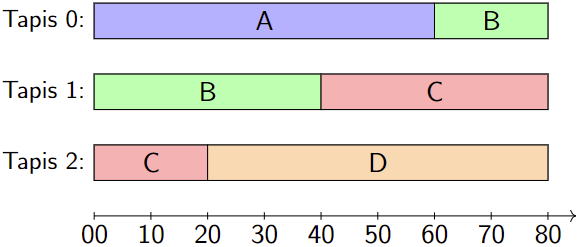
\includegraphics[width=60mm]{images/mcNaughton_output.png}
        \end{figure}
    \end{resolution}
    \comparison{
        \item optimal sur multi-processeur;
    }{
        \item faire des migrations;
        \item connaître tous les travaux;
    }
\end{definition}

\subsubsection*{Round-Robin}
\begin{definition}
    As the term is generally used, time slices, also known as time quanta, are assigned to each process in equal portions and in circular order, handling all processes without priority, also known as cyclic executive.
    \begin{example}
        Vous êtes seul et devez nourrir trois bébés. Lorsqu'un bébé attend sa cuillerée trop longtemps, il pleure. Dans quel ordre nourrissez vous les bébés? 
    \end{example}
    \comparison{
        \item simple;
        \item easy to implement;
    }{
        \item multiples préemptions prennent du temps CPU;
    }
\end{definition}

\subsubsection*{Multi-Level Feedback Queue}
\begin{definition}
    Amélioration de l'algorithme du Round-Robin avec plusieurs files qui change à partir de deux situations:
    \begin{enumerate}[noitemsep]
        \item \textbf{remonte} dans les priorités, quand un thread est:
        \begin{enumerate}[noitemsep]
            \item bloqué;
            \item attends depuis trop longtemps;
        \end{enumerate}
        \item \textbf{descend} dans les priorités, quand un thread est:
        \begin{enumerate}[noitemsep]
            \item utilise tout son quota de temps;
        \end{enumerate}
    \end{enumerate}
\end{definition}

\subsubsection*{Priorité Fixe}
\begin{definition}
    Un \textbf{Système Temps-Réel} est un système qui a la capacité de répondre à des évènements asynchrones issus du monde extérieur dans des délais pré-déterminés.
    \begin{phrase}
        temps-réel est différent de rapide
    \end{phrase}
    Généralement le système sera divise en deux types de tâches qui seront découper en différents threads:
    \begin{enumerate}[noitemsep]
        \item \textbf{Périodiques} déclenchement sur timer avec durée fixe;
        \item \textbf{Sporadiques} déclenchement sur interruption avec une durée minimale;
    \end{enumerate}
\end{definition}
\begin{definition}
    Algorithme d'Ordonnancement a Priorité Fixe
    \begin{theorem}
        Si on peut ordonnancer les tâches en priorité fixe, on saure le faire en affectant les priorités dans l'ordre inverse des périodes.
    \end{theorem}

    \begin{theorem}
        Si la charge du système est $<69\%$, alors les tâches sont ordonnançables en priorité fixe.
    \end{theorem}

    \begin{theorem}
        En monoprocesseur, tout système de tâche périodique faisable, charge processeur $<100\%$ est faisable avec l'algorithme EDF.        
    \end{theorem}

    \begin{remark}
        EDF reste optimal sur des tâches non périodiques. Connaissance des durées de calcul des tâches non nécessaire.
    \end{remark}    
    \begin{phrase}
        Il n'existe pas d'ordonnancement optimal en multi-processeur.
    \end{phrase}
\end{definition}


\subsection{Sécurité}
Quand on considère un Système d'Exploitation il faut toujours considère comment protéger des attaques externes et des conflits pour garantir l'intégrité du système:
\begin{definition}
    Découpage des fonctionnalités en processus indépendants en laissant les services: parties sensibles, minimales et incontournables.
\end{definition}
On utilise des \textbf{Principes de Sécurité de Saltzer et Schroeder} pour construire et évaluer la sécurité d'un OS:
\begin{enumerate}[rightmargin=\leftmargin]
    \item \textbf{Open Design}:
    \begin{definition}
        ne pas se reposer sur le fait que les attaquants ignoreront certains détails.
    \end{definition}

    \item \textbf{Psychological Acceptability}:
    \begin{definition}
        si la sécurité d'un système le rend trop pénible à utiliser, les utilisateurs contourneront les protections.
    \end{definition}

    \item \textbf{Work Factor}
    \begin{definition}
        Concevoir le système en évaluant les ressources d'un attaquant.
    \end{definition}
    
    \item \textbf{Compromise Recording}:
    \begin{definition}
        On peut parfois reporter son attention sur la détection d'une compromission plutôt que sur sa prévention.
    \end{definition}
\end{enumerate}
Pendant la construction d'OS il faut faire la séparation des privilèges en isolant les compromission de chaque partie du système.
\begin{remark}
    Il faut minimiser les mécanismes communs pour minimiser l'impact d'une compromission.
\end{remark}
Chaque parti du système sera responsable pour faire la séparation et protection:
\begin{enumerate}[noitemsep]
    \item \textbf{processus}: séparation des tâches en domaines de protection;
    \item \textbf{micro-noyau}: séparation des services en domaines de protections;
    \item \textbf{exo-noyau}: minimisation des noyau et services;
\end{enumerate}

\subsubsection{Gestion de Privilèges}
Au fur et à mesure que le système exécute ses fonctionnalités il faudrait avoir des utils pour gérer qui a accès à quoi. On se base toujours au \textbf{Principe du Moindre Privilège}:
\begin{definition}
    Principe du Moindre Privilège: autoriser seulement le nécessaire. Tout ce qui n'est pas explicitement autorisé est interdit.
\end{definition}
Pour bien identifier et localiser la relation entre les fichiers et les processus on considère:
\begin{enumerate}
    \item \textbf{processus}: associé à:
    \begin{enumerate}[noitemsep]
        \item un user id;
        \item un groupe id;
    \end{enumerate}
    
    \item \textbf{fichier}: associé à:
    \begin{enumerate}[noitemsep]
        \item un utilisateur;
        \item un groupe;
        \item les permissions:
        \begin{enumerate}[noitemsep]
            \item Read;
            \item Write;
            \item eXecute;
        \end{enumerate}
    \end{enumerate}
    Un fichier central associe les utilisateurs au groupe.
\end{enumerate}
Quand un fichier est ouvert, open, le noyau renvoie un numéro: le file descriptor qui sera utilisé pour les opérations sur le fichier.\\

Dans une système UNIX les permissions ne sont utilisées que pour l'ouverture du fichier. ensuite toutes les opérations sont faites en utilisant le file descriptor.\\

\subsubsection*{ACL}
Quand on considère une ressource il faudrait implementer une contrôle d'accès un \textbf{Access Control List, ACL}:
\begin{definition}
    \textbf{Access Control List} est une ensemble des listes de quels Processus peuvent faire quoi dans une Processeur.
\end{definition}
Avec les caractéristiques suivants:
\begin{enumerate}
    \item \textbf{Efficacité}:
    \begin{enumerate}[noitemsep]
        \item nécessite de mécanismes supplémentaires;
        \item un espace de nommage, nommer la ressource à laquelle on veut accéder;
        \item un mécanisme d'identification;
    \end{enumerate}

    \item \textbf{Responsabilité}, savoir qui peut avoir accès à quoi:
    \begin{enumerate}[noitemsep]
        \item la liste donne l'information directement;
    \end{enumerate}

    \item \textbf{Revocation}, supprimer l'accès:
    \begin{enumerate}[noitemsep]
        \item supprimer de la liste;
    \end{enumerate}
\end{enumerate}

\subsubsection*{Capacités}
Quand on considère une processus il faudrait implementer une liste de \textbf{Capacités}:
\begin{definition}
    \textbf{Capacités} est une liste de ce que une Processus peut faire pour chaque autre ressource d'un ordinateur.
\end{definition}
Avec les caractéristiques suivants:
\begin{enumerate}
    \item \textbf{Efficacité}:
    \begin{enumerate}[noitemsep]
        \item la capacité sert à nommer l'objet c'est un pointeur vers la ressource;
    \end{enumerate}

    \item \textbf{Responsabilité}, savoir qui peut avoir accès à quoi:
    \begin{enumerate}[noitemsep]
        \item peut être plus difficile;
    \end{enumerate}

    \item \textbf{Revocation}, supprimer l'accès:
    \begin{enumerate}[noitemsep]
        \item plus difficile: necessite de metre en place un proxy;
    \end{enumerate}
\end{enumerate}


\section{Multi-Tâche}

Quand on considère une OS il y aura Multi-Tâches qui se déroulent en même temps. On considère qu'une \textbf{Tâche} sera: 
\begin{definition}\label{def:tache}
    Terme ambigu, souvent synonyme de Processus mais parfois de Thread. Il faut faire attention à son utilisation.
\end{definition}

\subsection{Thread}
\begin{definition}\label{def:thread}
    Séquence d'exécution indépendante qui peut avoir des statuts suivants:
    \begin{figure}[H]
        \centering
        \begin{tikzpicture}[]
        
        \node[state, initial] (S0) {prt};
        \node[state, above right= of S0] (S1) {att};
        \node[state, below right= of S1] (S2) {exe};

        \draw[->] (S0) edge[bend left, below]  node{élection}    (S2);
        \draw[->] (S2) edge[bend left, below]  node{préparation} (S0);
        \draw[->] (S1) edge[bend right, left]  node{déblocage}   (S0);
        \draw[->] (S2) edge[bend right, right] node{blocage}     (S1);

        \end{tikzpicture}
    \end{figure}
    Où: prt est \textbf{prêt}, att est \textbf{en attente} et exe est \textbf{en exécution}.
    
    \begin{remark}
        L'Unité d'Ordonnancement est responsable pour ordonner les Threads.
    \end{remark}
\end{definition}

\subsubsection{Processus}
\begin{definition}\label{def:processus}
    L'Ensemble Threads et ses permissions, donc avec son espace d'adressage séparé.

    \begin{remark}
        En général une instance de l'exécution d'un programme est considère comme Processus.
    \end{remark}

    \begin{phrase}
        un processus peut être vu comme une \textbf{machine virtuelle} disposant de:
        \begin{enumerate}[noitemsep]
            \item \texttt{thread}: CPU virtuel;
            \item \texttt{espace d'adressage}: mémoire virtuelle;
            \item \texttt{périphériques virtuels}: permettent d'acceder des périphériques réels;
            \item \texttt{hyperviseur}: noyau virtuelle;
        \end{enumerate}
    \end{phrase}
\end{definition}

\subsubsection{Atomicité}
\begin{definition}\label{def:atomicite}
    \texttt{f} est \textbf{atomique} par rapport à \texttt{g} si \texttt{f} apparaît s'exécuter d'un seul coup sans être interrompue par l'exécution de \texttt{g}.\\

    Deux fonctions \texttt{f} et \texttt{g} sont atomiques si l'exécution entrelacée de \texttt{f} et \texttt{g} est équivalente à une exécution séquentielle de \texttt{f} puis \texttt{g} ou de \texttt{g} puis \texttt{f}.
\end{definition}


\subsection{Changement de Contexte}
\begin{definition}
    Consiste à sauvegarder en mémoire la valeur de tous les registres du thread en cours d'exécution, par exemple les données sur la pile, puis à restaurer les registres d'un thread dont les valeurs ont été précédemment sauvées.

    \begin{phrase}
        essentially suspending the process and then resuming it.
    \end{phrase}

    \begin{remark}
        Sert à implémenter plusieurs fils d'exécution, threads, indépendants sur un seul processeur.
    \end{remark}

    \begin{example}
        On suppose qu'on est en train de lire un livre. S'on est appelé pour faire un autre tâche plus important, on marque la page, fait la tâche et après on reprend là où on s'est arrêté pour continuer à lire.
    \end{example}
\end{definition}
S'il arrive un demande de changement de contexte pas immédiate le processus doit attendre qui le CPU prend connaissance de cette demande. Le CPU faire constamment du \textbf{Polling} pour découvrir s'il a besoin d'agir:
\begin{definition}
    The process in which the CPU constantly checks the status of the device to see if it needs the CPU's attention.
\end{definition}


\subsection{Interruptions}
Síl arrive un demande de changement de contexte immédiate le processus ira envoyer une \textbf{interruption}
\begin{definition}
    Mécanisme permettant de signaler au processeur un évènement requérant son attention immédiate.

    \begin{remark}
        Le \textbf{Interrupt Handler} c'est le service d'interruption qui est appellee comme réponse du processeur à une interruption.
    \end{remark}
\end{definition}
Lors d'une interruption il faut:
\begin{enumerate}[]
    \item \textbf{sauvegarder} les données anciennes:
    \begin{enumerate}[noitemsep]
        \item pc;
        \item sp;
    \end{enumerate}
    Généralement ce process est automatique et considère flags et d'autres registres utilises.

    \item \textbf{recevoir} les nouveaux valeurs:
    \begin{enumerate}[noitemsep]
        \item pc reçoit une adresse fixe qui dépend du numéro d'interruption;
        \item sp reçoit l'adresse d'une pile du noyau; 
    \end{enumerate}

    \item \textbf{exécution} de la routine;
    \item \textbf{restauration} de tous les registres du thread interrompu;
\end{enumerate}
Quand il y a une interruption pendant le traitement d'une autre interruption les nouvelles interruption sont masquées, ça veut dire que sont mises en attentes.
\begin{remark}
    Masquage des interruptions introduit de la latence dans le traitement des interruptions. Ainsi les interrupt handlers peuvent découper le traitement pour les exécuter plus rapidement.
\end{remark}
Sur Unix deux fonctions peuvent être utilises avec le changement de contexte:
\begin{enumerate}[rightmargin=\leftmargin]
    \item \textbf{mmap()}:
    \begin{definition}
        appel système UNIX permettant de projeter un fichier en mémoire qui récupère automatique une donnée, sur le disque dur, de la partie du fichier lors des défauts de page.
    \end{definition}
    
    \item \textbf{fork()}:
    \begin{definition}
        duplique un processus. initialement toute la mémoire est partagée entre les deux copies jusqu'à première modification qui modifiera l'accès aux pages partagées en lecture seule.
    \end{definition}
\end{enumerate}
Les Interruptions peuvent arriver de différent parties de l'ordinateur comme:
\begin{enumerate}[noitemsep, rightmargin=\leftmargin]
    \item \textbf{Interruptions Matérielles}:
    \begin{definition}
        Interruptions qui provient d'un périphérique matériel.
    \end{definition}
    Comme:
    \begin{enumerate}[noitemsep]
        \item entrée clavier;
        \item arrivée d'un paquet réseau;
        \item fin de traitement d'une lecture ou écriture disque;
    \end{enumerate}
    \begin{remark}
        Programmée d'une Horloge est nomme \textbf{timer} en anglais.
    \end{remark}
    
    \item \textbf{Interruptions Logicielles}
    \begin{definition}
        Interruptions qui provient du processeur lui-même.
    \end{definition}
    Comme:
    \begin{enumerate}[noitemsep]
        \item division par zéro;
        \item accès à une zone mémoire interdit ou impossible;
        \item interruptions volontaires;
    \end{enumerate}
    \begin{remark}
        Interruptions Volontaires est nomme \textbf{trap} en anglais.
    \end{remark}
\end{enumerate}

\subsubsection{Préemption}
\begin{definition}
    Après une interruption un contexte différent est restauré au lieu du courant.
    \begin{remark}
        Interruptions sont le mécanisme matériel à la base de l'Ordonnancement Préemptif.
    \end{remark}
\end{definition}



\subsection{Synchronisation}
\begin{definition}\label{def:synchronisation}
    Mécanismes permettant de coordonner l'exécution de plusieurs threads en bloquant leur exécution à des points de programmes précis pour régler les problèmes de concurrence sur l'accès à une ressource, logicielle ou matérielle, partagée.

    \begin{remark}
        Bloquer c'est à dire changer le statut de tâches à bloqué.
    \end{remark}
    \begin{remark}
        Débloquer c'est à dire changer le statut des taches à prêt.
    \end{remark}
\end{definition}
Pendant le changement entre threads la CPU restera inactif pour un des threads et donc perdra du temps d'exécution. Il faut copier les adresses de mémoire nécessaires que prend un peu de temps. On considère les méthodes de synchronisation suivants:
\begin{enumerate}[noitemsep, rightmargin=\leftmargin]
    \item \texttt{mutex}:
    \begin{definition}\label{def:mutex}
        Utilisation de code qui permet de gérer des conflit pour ressources. 
    \end{definition}
    
    \item \textbf{Concurrence}:
    \begin{definition}\label{def:concurrence}
        Quand les tâches accèdent simultanément à une même ressource.
    \end{definition}
    
    \item \textbf{Parallélisme}:
    \begin{definition}\label{def:parallelisme}
        Quand il y a utilisation de plusieurs resources.
    \end{definition}
\end{enumerate}



% \section{Travail Dirigé}
% \subsection{Séance 07/11/2022}
% \paragraph{Définition}Dans ce TD on avait besoin de comprendre la structure et adresse de mémoire. Ainsi on considère le code suivant:
% \begin{scriptsize}\mycode
%     \begin{lstlisting}[language=C]
%     struct p {
%         uint32_t x; // 32 bits -> 4 octets
%         uint16_t u; // 16 bits -> 2 octets
%         uint32_t y; // 32 bits -> 4 octets
%         uint32_t z; // 32 bits -> 4 octets
%     } __attribute__((packed));;

%     struct p *prt;
%     \end{lstlisting}
% \end{scriptsize}
% Le \texttt{packed} assure que les champs des structures sont les uns à la suite des autres, donc il n'aura pas de \textbf{padding} pendant l'execution du code. Si \texttt{prt} point à l'adresse 0x1000 alors:
% \begin{enumerate}[noitemsep]
%     \item \texttt{\&(ptr->x)} pointe à l'adresse 0x1000
%     \item \texttt{\&(ptr->u)} pointe à l'adresse 0x1004
%     \item \texttt{\&(ptr->y)} pointe à l'adresse 0x1006
%     \item \texttt{\&(ptr->z)} pointe à l'adresse 0x100A
% \end{enumerate}
% On rapelle que 0x represente des numéros hexadecimales.

% \newpage\subsection{Séance 14/11/2022}
% \paragraph{Définition}16 kilo octets = 16 kilo bytes = 16 000 bytes
% dans le td il faut faire la plut part hardcoded
% char *heap c'est un tableau de pointeurs et char heap c'est un tableau de char
% memalloc doit reçu

% \newpage\subsection{Séance 21/11/2022}
% \paragraph{Définition}Dans ce TD on avait besoin de comprendre des \texttt{threads} coopératifs. Il faudra link les fichiers C et assembleur avec les options de compilateur \texttt{-static} comme montre:
% \begin{scriptsize}\mycode
%     \begin{lstlisting}[language=Bash]
%         gcc -static file.s main.c -o main.exe
%         ./main.exe
%     \end{lstlisting}
% \end{scriptsize}
% On note que c'est nécessaire declarer des fonctions en Assemble avec les codes suivants:
% \begin{scriptsize}\mycode
%     \lstinputlisting[language=C, linerange={1-5}]{TD/2022_11_21/main.c}
% \end{scriptsize}
% \begin{scriptsize}\myRISCV
%     \lstinputlisting[linerange={1-5}]{TD/2022_11_21/utils.s}
% \end{scriptsize}

% \newpage\subsection{Séance 28/11/2022}
% \paragraph{Définition}Dans ce TD on avait besoin de comprendre des \texttt{interruptions} et le \texttt{ordonnancement} des instructions.
% \begin{scriptsize}\mycode
%     \lstinputlisting[language=C, linerange={1-5}]{TD/2022_11_28/main.c}
% \end{scriptsize}
% % gcc -static utils.s -g main.c -o main.exe
% % gdb ./main.exe
% % break enter_coroutine
% % run
% % n
% % Thread 1 received signal SIGSEGV, Segmentation fault.

% \newpage\subsection{Séance 05/12/2022}
% \paragraph{Définition}
% \begin{scriptsize}\mycode
%     \lstinputlisting[language=C, linerange={1-5}]{TD/2022_12_05/main.c}
% \end{scriptsize}
\end{document}